\documentclass[letterpaper,11pt]{memoir}
  \usepackage[utf8]{inputenc}
  \usepackage{fourier,microtype}       % texte en Utopia
  \usepackage[scaled=0.82]{beramono}   % code en Bera
  \renewcommand{\sfdefault}{Myriad-LF} % titres en MyriadPro
  \usepackage{natbib,url}
  \usepackage[english,francais]{babel}
  \usepackage[autolanguage]{numprint}
  \usepackage{vgmath,actu,amsmath,amsthm,amsfonts,icomma}
  \usepackage[noae]{Sweave}
  \usepackage{paralist}
  \usepackage[shortlabels]{enumitem}
  \usepackage{textpos}
  \usepackage{graphicx,color,soulutf8}
  \usepackage{manfnt}                  % \mantriangleright (puce)
  \usepackage{marvosym}                % \Forward
  \usepackage{applekeys}               % touches Mac
  \usepackage{listingsutf8,answers}
  \usepackage{pdfpages}                % couvertures

  %%%  Couleurs
  \definecolor{comments}{rgb}{0.7,0,0}
  \definecolor{shadecolor}{gray}{0}
  \definecolor{link}{rgb}{0,0,0.4}
  \definecolor{darkblue}{rgb}{0,0,0.75}

  %%% Hyperliens
  \usepackage{hyperref}
  \hypersetup{colorlinks,allcolors=link}

  %%% ============
  %%%  Page titre
  %%% ============
  \title{%
    \fontseries{b}\fontsize{42}{33}\selectfont ACT 2002 \\
    \fontseries{m}\fontsize{32}{33}\selectfont Méthodes numériques \\
                                               en actuariat \\[20mm]
    \fontseries{b}\fontsize{36}{36}\selectfont Partie I \\
    \fontseries{m}\fontsize{32}{36}\selectfont Programmation en R}
  \author{%
    \fontseries{b}\fontsize{16}{20}\selectfont Vincent Goulet \\
    \fontseries{m}\fontsize{14}{18}\selectfont Professeur titulaire \textbar\
                                               École d'actuariat \textbar\
                                               Université Laval}
  \date{%
    \fontseries{m}\fontsize{14}{18}\selectfont Notes de cours \textbar\
                                               Exercices \textemdash\
                                               édition 2013}

  %%% ===================
  %%%  STYLE DU DOCUMENT
  %%% ===================

  %% Titres des chapitres
  \chapterstyle{hangnum}
  \renewcommand{\chaptitlefont}{\normalfont\Huge\sffamily\bfseries\raggedright}

  %% Marges, entêtes et pieds de page
  \setlength{\marginparsep}{7mm}
  \setlength{\marginparwidth}{13mm}
  \setlength{\headwidth}{\textwidth}
  \addtolength{\headwidth}{\marginparsep}
  \addtolength{\headwidth}{\marginparwidth}

  %% Titres des sections et sous-sections
  \setsecheadstyle{\normalfont\Large\sffamily\bfseries\raggedright}
  \setsubsecheadstyle{\normalfont\large\sffamily\bfseries\raggedright}
  \maxsecnumdepth{subsection}
  \setsecnumdepth{subsection}

  %% Listes. Paramétrage avec enumitem.
  \setlist[enumerate]{leftmargin=*,align=left}
  \setlist[enumerate,2]{label=\alph*),labelsep=*,leftmargin=1.5em}
  \setlist[enumerate,3]{label=\roman*),labelsep=0.5em,align=right}
  \setlist[itemize]{leftmargin=*,align=left}
  % \setenumerate{leftmargin=*,align=left}
  % \setenumerate[2]{label=\alph*)}
  % \setenumerate[3]{label=\roman*),align=right}
  % \setitemize{leftmargin=*,align=left}

  %% Noms de fonctions, code, etc.
  \newcommand{\code}[1]{\texttt{#1}}

  %% Environnements d'exemples et al.
  \theoremstyle{definition}
  \newtheorem*{astuce}{Astuce}

  %% Options de babel
  \frenchbsetup{CompactItemize=false,%
    ThinSpaceInFrenchNumbers=true,
    ItemLabeli=\mantriangleright,
    ItemLabelii=\textendash}
  \addto\captionsfrench{\def\figurename{{\scshape Fig.}}}
  \addto\captionsfrench{\def\tablename{{\scshape Tab.}}}

  %%% =========================
  %%%  Nouveaux environnements
  %%% =========================

  %% Listes d'objectifs au début des chapitres
  \newenvironment{objectifs}{%
    \noindent
    \begin{framed}
      \vspace{-1.33\baselineskip}
      \begin{shaded}
        \noindent\sffamily\bfseries\textcolor{white}{Objectifs du chapitre}
      \end{shaded}
      \vspace{-0.6\baselineskip}
      \setlength{\labelsep}{1ex}
      \settowidth{\labelwidth}{\mantriangleright}
      \setlength{\leftmargini}{\labelwidth}
      \addtolength{\leftmargini}{\labelsep}
      \begin{compactitem}
        \small}
      {\end{compactitem}
    \end{framed}}

  %% Environnements de Sweave
  \DefineVerbatimEnvironment{Sinput}{Verbatim}{xleftmargin=\parindent}
  \DefineVerbatimEnvironment{Soutput}{Verbatim}{xleftmargin=\parindent}
  \DefineVerbatimEnvironment{Scode}{Verbatim}{xleftmargin=\parindent}
  \fvset{listparameters={\setlength{\topsep}{0pt}}}
  \renewenvironment{Schunk}{\vspace{\topsep}}{\vspace{\topsep}}

  %% Exercices et réponses
  \Newassociation{rep}{reponse}{reponses}
  \newcounter{exercice}[chapter]
  \newenvironment{exercice}{%
    \begin{list}{\bfseries \thechapter.\arabic{exercice}}{%
        \refstepcounter{exercice}
        \settowidth{\labelwidth}{\bfseries \thechapter.\arabic{exercice}}
        \setlength{\leftmargin}{\labelwidth}
        \addtolength{\leftmargin}{\labelsep}
        \setlist[enumerate,1]{label=\alph*),labelsep=*,leftmargin=1.5em}
        \setlist[enumerate,2]{label=\roman*),labelsep=0.5em,align=right}}
      \item}
    {\end{list}}
  \renewenvironment{reponse}[1]{%
    \begin{enumerate}[label=\textbf{#1}]
      \item}
    {\end{enumerate}}
  % \renewenvironment{reponse}[1]{%
  %   \begin{enumerate}[label=#1,font=\bfseries]
  %     \setenumerate[2]{leftmargin=*,labelsep=0em}
  %     \item}
  %   {\end{enumerate}}
  \renewcommand{\reponseparams}{{\thechapter.\theexercice}}

  %% Listes de commandes
  \newenvironment{ttscript}[1]{%
    \begin{list}{}{%
        \setlength{\labelsep}{1.5ex}
        \settowidth{\labelwidth}{\fbox{\code{#1}}}
        \setlength{\leftmargin}{\labelwidth}
        \addtolength{\leftmargin}{\labelsep}
        \setlength{\parsep}{0.5ex plus0.2ex minus0.2ex}
        \setlength{\itemsep}{0.3ex}
        \renewcommand{\makelabel}[1]{\fbox{##1}\hfill}}}
    {\end{list}}

  %% Chapitre Opérateurs: environnements pour placer côte à côte des
  %% définitions de fonctions (utilisant ttscript ci-dessus) et un
  %% petit exemple.
  \newenvironment{operateur}[1]{%
    \noindent
    \begin{minipage}[t]{0.65\linewidth}
      \begin{ttscript}{#1}}
    {\end{ttscript}\end{minipage}\hfill}
  \newenvironment{miniexemple}{%
    \begin{minipage}[t]{0.3\linewidth}}
    {\end{minipage}}

  %%% Listes de structures de contrôle
  \newenvironment{struclist}{%
    \begin{description}[style=nextline,font=\mdseries\ttfamily]}
    {\end{description}}

  %%% Remarques importantes
  \newenvironment{important}{%
    \begin{framed}%
      \noindent
      \begin{minipage}{0.1\linewidth}
        \raisebox{-0.5em}[0em][0em]{\LARGE\danger}
      \end{minipage}
      \begin{minipage}[t]{0.85\linewidth}}
      {\end{minipage}%
    \end{framed}}

  %%% =====================
  %%%  Nouvelles commandes
  %%% =====================

  %%% Indications de capsule vidéo
  \setulcolor{darkblue}
  \setul{1.5pt}{0.7pt}
  \newcommand{\video}{%
    $\mathrel{\vcenter{\offinterlineskip%
        \color{darkblue}
        \fontsize{32}{32}\selectfont
        \hbox{$\bigcirc$}%
        \fontsize{24}{22}\selectfont\vskip-20.4pt\hskip8.5pt
        \hbox{\Forward}}}$}
  \newcommand{\capsule}[1]{\marginpar{\video}\ul{#1}}


  %%% =============================================
  %%%  Paramètres pour les sections de code source
  %%% =============================================
  \lstloadlanguages{R}
  \lstdefinelanguage{Renhanced}[]{R}{%
    morekeywords={colMeans,colSums,head,is.na,is.null,mapply,ms,na.rm,%
      nlmin,replicate,row.names,rowMeans,rowSums,sys.time,system.time,%
      tail,which.max,which.min},
    deletekeywords={c},
    alsoletter={.\%},%
    alsoother={:_\$}}
  \lstset{language=Renhanced,
    extendedchars=true,
    inputencoding=utf8/latin1,
    basicstyle=\small\ttfamily,
    commentstyle=\color{comments}\slshape,
    keywordstyle=\mdseries,
    showstringspaces=false,
    index=[1][keywords],
    indexstyle=\indexfonction}

  %%% =======
  %%%  Index
  %%% =======
  \newcommand{\bfhyperpage}[1]{\textbf{\hyperpage{#1}}}
  \renewcommand{\preindexhook}{%

    Les numéros de page en caractères gras indiquent les pages où les
    concepts sont introduits, définis ou expliqués.\vskip\onelineskip}
  \newcommand{\Index}[1]{\index{#1|bfhyperpage}}
  \newcommand{\indexargument}[1]{\index{#1@\code{#1}}}
  \newcommand{\Indexargument}[1]{\Index{#1@\code{#1}}}
  \newcommand{\indexattribut}[1]{\index{#1@\code{#1} (attribut)}}
  \newcommand{\Indexattribut}[1]{\Index{#1@\code{#1} (attribut)}}
  \newcommand{\indexclasse}[1]{\index{#1@\code{#1} (classe)}}
  \newcommand{\Indexclasse}[1]{\Index{#1@\code{#1} (classe)}}
  \newcommand{\indexfonction}[1]{\index{#1@\code{#1}}}
  \newcommand{\Indexfonction}[1]{\Index{#1@\code{#1}}}
  \newcommand{\indexmode}[1]{\index{#1@\code{#1} (mode)}}
  \newcommand{\Indexmode}[1]{\Index{#1@\code{#1} (mode)}}
  \newcommand{\indexobjet}[1]{\index{#1@\code{#1}}}
  \newcommand{\Indexobjet}[1]{\Index{#1@\code{#1}}}
  \newcommand{\indexemacs}[1]{\index{Emacs!#1@\texttt{#1}}}
  \newcommand{\indexess}[1]{\index{ESS!#1@\texttt{#1}}}

  \newcommand{\attribut}[1]{\code{#1}\indexattribut{#1}}
  \newcommand{\Attribut}[1]{\code{#1}\Indexattribut{#1}}
  \newcommand{\argument}[1]{\code{#1}\indexargument{#1}}
  \newcommand{\Argument}[1]{\code{#1}\Indexargument{#1}}
  \newcommand{\classe}[1]{\code{#1}\indexclasse{#1}}
  \newcommand{\Classe}[1]{\code{#1}\Indexclasse{#1}}
  \newcommand{\fonction}[1]{\code{#1}\indexfonction{#1}}
  \newcommand{\Fonction}[1]{\code{#1}\Indexfonction{#1}}
  \newcommand{\mode}[1]{\code{#1}\indexmode{#1}}
  \newcommand{\Mode}[1]{\code{#1}\Indexmode{#1}}
  \newcommand{\objet}[1]{\code{#1}\indexobjet{#1}}
  \newcommand{\Objet}[1]{\code{#1}\Indexobjet{#1}}
  \newcommand{\emacs}[1]{\code{#1}\indexemacs{#1}}
  \newcommand{\ess}[1]{\code{#1}\indexess{#1}}
  \makeindex

  %%% Sous-figures
  \newsubfloat{figure}

  %%% Style de la bibliographie
  \bibliographystyle{francais}

  %%% Aide pour la césure
  \hyphenation{con-sole}

%  \includeonly{emacs+ess}

\begin{document}

\frontmatter

\pagestyle{empty}

%% Page couverture avant. Il faut modifier la largeur des graphiques
%% puisque Sweave la règle à 0.8\textwidth.
\setkeys{Gin}{width=\paperwidth}
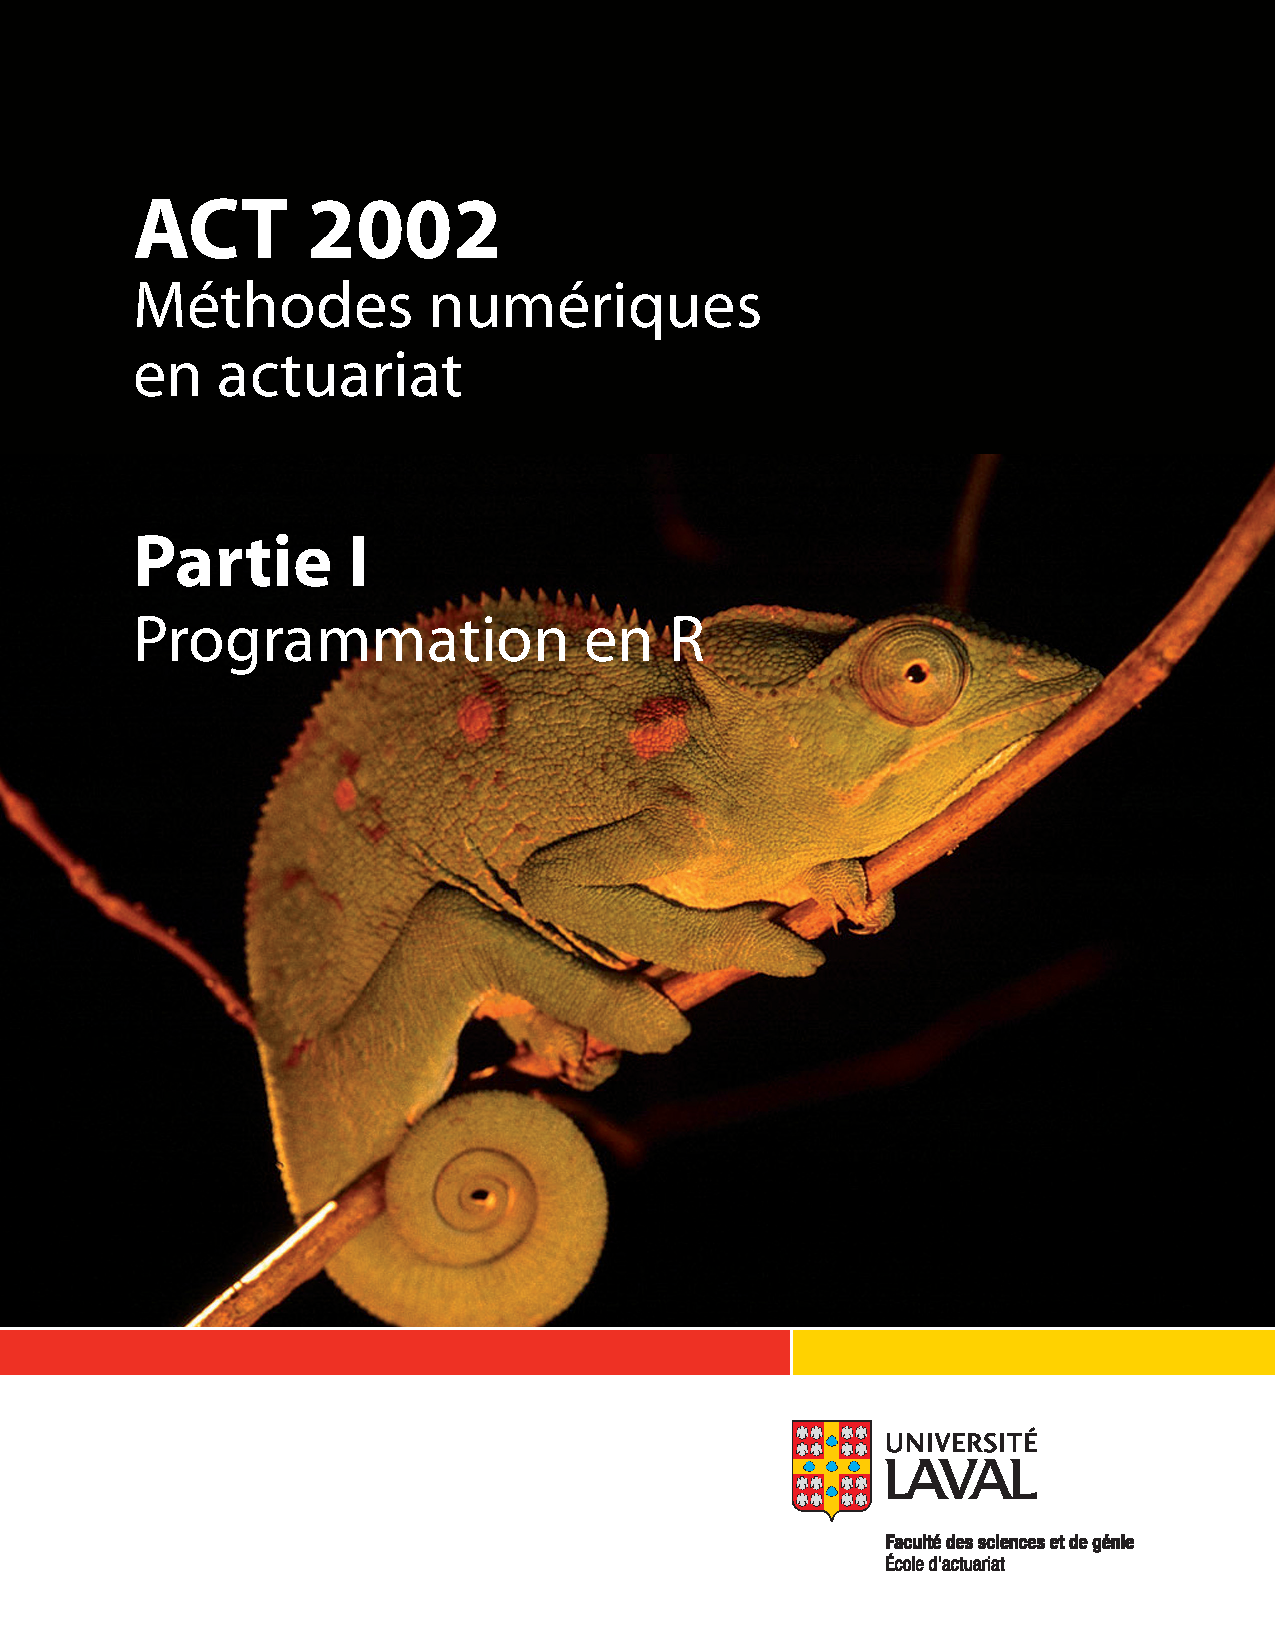
\includepdf[pages=1]{couvertures-partie_1}
\setkeys{Gin}{width=0.8\textwidth}
\cleardoublepage

\begin{adjustwidth*}{-12mm}{-72mm}
  \sffamily
  \raggedright
  \vspace*{-17mm}
  \thetitle \\
  \vspace*{20mm}
  \theparttitle \\
  \vspace*{32mm}
  \theauthor \\
  \vspace*{\fill}
  \thedate
\end{adjustwidth*}

%%% Local Variables:
%%% mode: latex
%%% TeX-master: "methodes_numeriques-partie_3"
%%% coding: utf-8
%%% End:

\clearpage

\begingroup
\calccentering{\unitlength}
\begin{adjustwidth*}{\unitlength}{-\unitlength}
  \setlength{\parindent}{0pt}
  \setlength{\parskip}{\baselineskip}

  {\textcopyright} {\year} Vincent Goulet \\

  
\includegraphics[height=7mm,keepaspectratio=true]{../share/by-sa}\\%
Cette création est mise à disposition selon le contrat
\href{http://creativecommons.org/licenses/by-sa/4.0/deed.fr}{%
  Attribution-Partage dans les mêmes conditions 4.0 International} de
Creative Commons. En vertu de ce contrat, vous êtes libre de:
\begin{itemize}
\item \textbf{partager} --- reproduire, distribuer et communiquer
  l'{\oe}uvre;
\item \textbf{remixer} --- adapter l'{\oe}uvre;
\item utiliser cette {\oe}uvre à des fins commerciales.
\end{itemize}
Selon les conditions suivantes:

\begin{tabularx}{\linewidth}{@{}lX@{}}
  \raisebox{-9mm}[0mm][13mm]{%
    
\includegraphics[height=11mm,keepaspectratio=true]{../share/by}} &
  \textbf{Attribution} --- Vous devez créditer l'{\oe}uvre, intégrer
  un lien vers le contrat et indiquer si des modifications ont été
  effectuées à l'{\oe}uvre. Vous devez indiquer ces informations par
  tous les moyens possibles, mais vous ne pouvez suggérer que
  l'Offrant vous soutient ou soutient la façon dont vous avez utilisé
  son {\oe}uvre. \\
  \raisebox{-9mm}{
\includegraphics[height=11mm,keepaspectratio=true]{../share/sa}}
  & \textbf{Partage dans les mêmes conditions} --- Dans le cas où vous
  modifiez, transformez ou créez à partir du matériel composant
  l'{\oe}uvre originale, vous devez diffuser l'{\oe}uvre modifiée dans
  les même conditions, c'est à dire avec le même contrat avec lequel
  l'{\oe}uvre originale a été diffusée.
\end{tabularx}


  \textbf{Code source} \\
  Le code source {\LaTeX} et R de ce document est disponible à l'adresse
    \url{https://svn.fsg.ulaval.ca/svn-pub/vgoulet/documents/methodes_numeriques/}
  ou en communiquant directement avec l'auteur.

  \textbf{Couverture} \\
  Le reptile en couverture est un caméléon tapis (\emph{Furcifer
    lateralis}) originaire de Madagascar. Adulte, sa taille atteint
  les 25~cm, queue comprise.

  Crédit photo: Michabln Schwarz; \url{http://fc-foto.de/2077174}
\end{adjustwidth*}
\endgroup

%%% Local Variables:
%%% mode: latex
%%% TeX-master: "methodes_numeriques-partie_4"
%%% coding: utf-8
%%% End:

\clearpage

\pagestyle{companion}

\chapter*{Introduction}
\addcontentsline{toc}{chapter}{Introduction}
\markboth{Introduction}{Introduction}

Il existe de multiples ouvrages traitant de l'environnement
statistique R. Dans la majorité des cas, toutefois, le logiciel est
présenté dans le cadre d'applications statistiques spécifiques. Ce
document se concentre plutôt sur l'apprentissage du langage de
programmation sous-jacent aux diverses fonctions statistiques, langage
lui aussi nommé R.

Chaque chapitre présente en rafale plusieurs éléments de théorie avec
généralement peu d'exemples. La lecture d'un chapitre permet donc
d'acquérir rapidement plusieurs nouvelles connaissances sur le langage
R. Cependant, pour compléter son apprentissage, le lecteur devra aussi
étudier attentivement et, surtout, exécuter ligne par ligne le code R
fourni dans les sections d'exemples à la fin des chapitres (sauf un).
Ces sections d'exemples couvrent l'essentiel des concepts présentés
dans les chapitres et les complémentent souvent. L'étude de ces
sections fait partie intégrante de l'apprentissage du langage R.

Le code des sections d'exemples est disponible dans le site du cours.
Nous fournissons également des fichiers de sortie contenant les
résultats de chacune des expressions.

Un symbole de lecture vidéo dans la marge, tel que ci-contre, indique
qu'une capsule vidéo sur \capsule{le sujet} identifié par la marque de
soulignement est disponible dans le site du cours.

Certains exemples et exercices font référence à des concepts de base
de la théorie des probabilités et des mathématiques financières. Les
contextes actuariels demeurent néanmoins peu nombreux et ne devraient
généralement pas dérouter le lecteur pour qui ces notions sont moins
familières. Les réponses de tous les exercices se trouvent en annexe.

On trouvera également en annexe une brève introduction à l'éditeur de
texte GNU~Emacs et au mode ESS, ainsi qu'une présentation sur
l'administration d'une bibliothèque de packages R.

Je tiens à remercier M.~Mathieu Boudreault pour sa collaboration
dans la rédaction des exercices.

%%% Local Variables:
%%% mode: latex
%%% TeX-master: "methodes_numeriques-partie_1"
%%% coding: utf-8
%%% End:

\cleartorecto
\tableofcontents*

\mainmatter
\include{presentation}
\include{bases}
\include{operateurs}
\include{exemples}
\include{fonctions}
\include{avance}

\appendix
\include{emacs+ess}
\include{packages}
\chapter{Réponses des exercices}
\label{reponses}
\markboth{Réponses des exercices}{Réponses des exercices}

\input{solutions-bases}
\input{solutions-operateurs}
\input{solutions-exemples}
\input{solutions-fonctions}
\input{solutions-avance}

%%% Local Variables:
%%% mode: latex
%%% TeX-master: "methodes_numeriques-partie_1"
%%% coding: utf-8
%%% End:
     % différent de Introduction à la...

\bibliography{r,stat,informatique}

\cleardoublepage
\printindex

\thispagestyle{empty}
\vspace*{\fill}

\begingroup
\calccentering{\unitlength}
\begin{adjustwidth*}{\unitlength}{-\unitlength}
  \begin{flushleft}
    \small %
    Ce document a été produit avec le système de mise en page
    {\XeLaTeX}. Le texte principal est en Lucida Bright~OT 11~points,
    les mathématiques en Lucida Bright Math~OT, le code informatique
    en Lucida Grande Mono~DK et les titres en Adobe Myriad~Pro. Des
    icônes proviennent de la police Font~Awesome. Les graphiques ont
    été réalisés avec R.
  \end{flushleft}
\end{adjustwidth*}
\endgroup
\vfill


\cleardoublepage
\cleartoverso

%% Page couverture arrière.
\setkeys{Gin}{width=\paperwidth}
\includepdf[pages=2]{couvertures-partie_1}

\end{document}

%%% Local Variables:
%%% mode: latex
%%% TeX-master: t
%%% coding: utf-8
%%% End:
